\chapter{Coordinate Frames}
\label{sec:CoordianteFrames}

A very crucial part of this project, was the analysis of the MAV's coordinate systems. This is very important because the MAV takes its desired position from what it detects from its camera and has to the controller's reference frame with respect to the world frame. Furthermore, the apriltag's position in the simulated world is defined by it's pose as detected from the usb camera. For the transformations the ASL's minkindr library was used. It should be noted, that the color coding in the axes frames follows the RVIZ color convention, meaning blue defines the z axis, green the y axis and red the x axis respectively. Furthermore the ASL's frame naming convention \cite{FrameNamingConvention} is followed throughout this project. 

 \section{Coordinate Frames in the Simulation }
 \label{sec: CoordinatesinSimulation}
 
 The first thing that should be resolved in the simulation world, was the correct positioning of the apriltag with respect to the usb camera detection. Although the two frames share the same origin point, the have different orientations as seen by figure \ref{pics:worldcamframe}, the distance between the two frames is set to emphasize the rotation. As it can easily be seen the transformation form camera frame to the world frame consists of one rotation of $90^{\circ}$ around the y axis $(rot_{y}(90^{\circ}))$ and a successive rotation of $-90^{\circ}$ around the axis $(rot_z(-90^{\circ}))$ as presented in the equation \ref{eq:camtoworldrot}. With the aforementioned transformation, the coordinates as seen from the camera match the actual world coordinates. Furthermore, it is easily understood that the apriltag's yaw in the real world corresponds to the negative pitch of the detected image.
 
  \begin{equation}
  \label{eq:camtoworldrot}
  \left[\begin{array}{c}
  x_{wc} \\ y_{wc} \\ z_{wc}  \end{array} \right] = Rot_{y}(90^{\circ})Rot_z(-90^{\circ})\left[ \begin{array}{c} x_c \\ y_c \\z_c \end{array} \right]
  \end{equation}
 
  
 %\begin{equation}
 %\label{eq:camtoworldrot}
 %\left[\begin{array}{c}
 %x_{wc} \\ y_{wc} \\ z_{wc}  \end{array} \right] = %Rot_{y}(90^{\circ})Rot_z(-90^{\circ})\left[ \begin{array}{c} x_c \\ y_c \\z_c %\end{array} \right] = \begin{bmatrix} 0 & 0 & 1 \\ -1 & 0 & 0 \\ 0 & -1 & 0 %\end{bmatrix} \left[ \begin{array}{c} x_c \\ y_c \\z_c \end{array} \right]
 %\end{equation}
  
  
 \begin{figure}
    \centering
    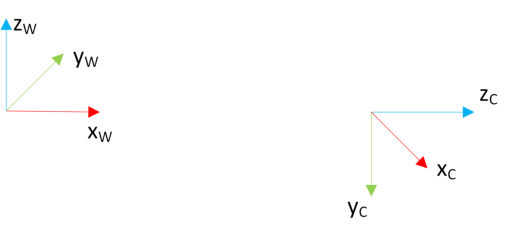
\includegraphics[width=0.98\textwidth]{images/world_camera_frame.pdf}
    \caption{The camera frame and the world frame.}
    \label{pics:worldcamframe}
 \end{figure}
 
 After the transformation of the camera frame, now come the coordinate transformations regarding the MAV. The transformation between the MAV's body frame and the world frame is obtained by subscribing to the firefly's odometry sensor, in the simulation it is named as odometry\textunderscore sensor1, the obtained transformation is represented by $T_{W\textunderscore B}$. Then the static transform between the body frame and the onboard camera frame is provided as parameter by the configuration file and is represented as $T_{B\textunderscore C}$. The aforementioned transform is passed as parameter in order to reduce the calculations needed to be perform and thus, speed up the procedure. The transformation between the MAV's camera and the Apriltag is obtained by subscribing to the MAV's  tag\textunderscore detection\textunderscore pose topic. This provides the pose of the detected Apriltag with respect to the camera coordinate frame. Now the last part was to obtain the transformation between the Apriltag frame and the reference frame. As it can be seen from the \ref{pics:mavcoordinateframe} the reference frame has the same orientation as the world system and is translated from it by the offsets specified by the user in the parameters' file. The transformation between the apriltag frame with respect to the reference frame can be seen from the image \ref{pics:mavcoordinateframe}, while the rotation is composed by a rotation around the y axis by $-90^{\circ}$ and a rotation around the z axis by $90^{\circ}$.The offsets, and especially the offset in the x axis since this defines the straight distance between the MAV and the Tag, are added so as to ensure that the MAV will keep a safety distance between itself and the Apriltag. If the x offset is set to zero, then the reference frame coincides with the Tag's frame, and they will collide, since the reference position of the MAV is set to the exact equal coordinates of the Tag. The aforementioned are presented in equation \ref{TRA}. The final coordinates that are sent to the controller are the result of the transformation presented in equation \ref{TWR} and they express the reference frame coordinates with respect to the world frame.
 
 
 \begin{equation}
 \label{TRA}
 T_{R\textunderscore A} = Rot_y(-90^{\circ}) * Rot_z(90^{\circ}) * \left[\begin{array}{c}
 x_A\\ y_A \\z_A
 \end{array}\right] + \left[\begin{array}{c}offset\textunderscore x \\ offset\textunderscore y \\offset\textunderscore z \\ \end{array}\right]
 \end{equation}
 
 
 
 \begin{equation}
 \label{TWR}
 T_{W\textunderscore R} = T_{W\textunderscore B} * T_{B\textunderscore C} * T_{C\textunderscore A} * {T_{R\textunderscore A}}^{-1}
 \end{equation}  
 
  \begin{figure}
     \centering
     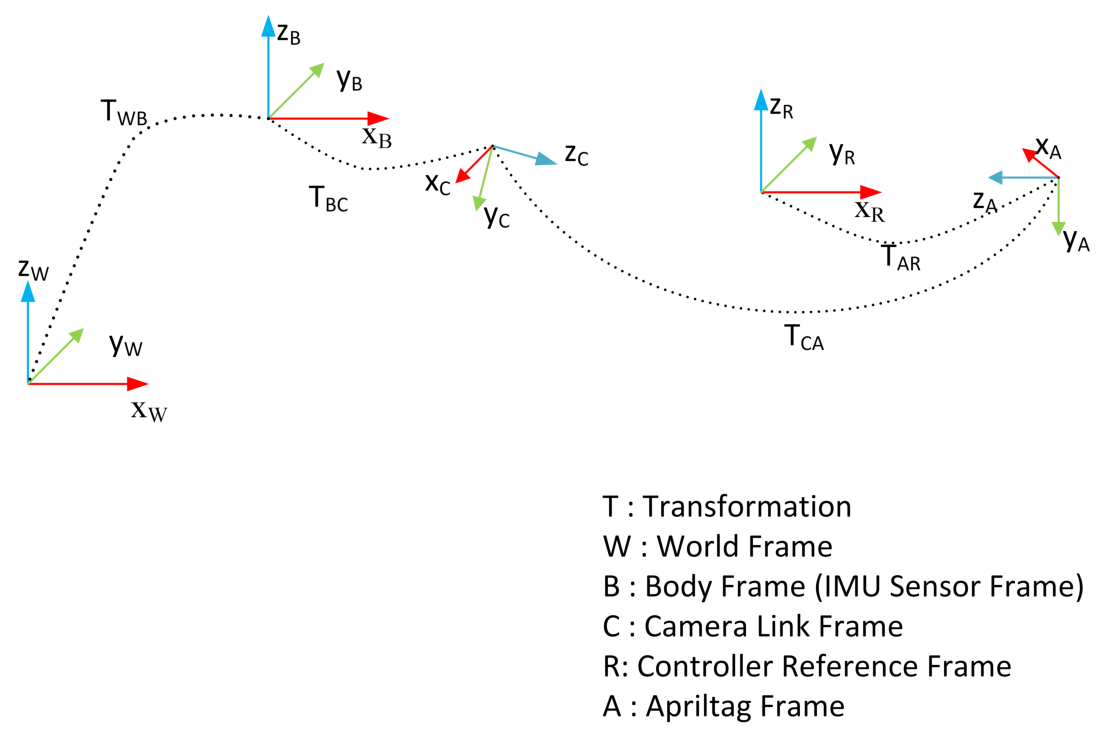
\includegraphics[width=0.99\textwidth]{images/coordinate_frame_representation_v3.pdf}
     \caption{The camera frame and the world frame.}
     \label{pics:mavcoordinateframe}
  \end{figure}
  
  
\section{Coordinate Frames in the Real System}
\label{sec: CoordinatesinRealSystem}
  